\chapter[Algoritmos Analisados]{Algoritmos Analisados}
\label{benchmarking}

O terceiro objetivo deste trabalho é a implementação da política de alguns algoritmos de RRA para que seus desempenhos possam ser analisados. Neste capítulo, iremos apresentar os quatro algoritmos que foram escolhidos para serem implementados no nosso ambiente de simulação. 

Os algoritmos selecionado foram propostos em \citeonline{Phd:Song2005}, \citeonline{Proc:Lei2007}, \citeonline{Nasralla2013} e \citeonline{basukala2009performance}.
Esses algoritmos foram escolhidos primeiramente devido à compatibilidade da implementação deles com o modelo de simulação considerado neste trabalho. Outro motivo para essa escolha foi que os autores desses algoritmos mostraram em seus respectivos trabalhos que esses algoritmos superaram os algoritmos de RRA clássicos EXP, MLWDF, PF.

Uma das ferramentas que pode ser utilizada para a concepção de algoritmos de RRA é a teoria da utilidade, a qual foi utilizada para ambientes com serviço único em \citeonline{Art:Song2005_Commag}, \citeonline{lei2007qos}, \citeonline{Proc:Ryu2005}, \citeonline{Rodrigues2014_Wiley}, e para cenários com múltiplos serviços em \citeonline{Phd:Song2005} e  \citeonline{Proc:Lei2007}. Essa teoria foi inicialmente concebida para aplicações na área da economia, onde era utilizada para tentar explicar o comportamento de um determinado consumidor e ajudar no processo decisório \cite{fishburn1968utility,north1968tutorial}. No entanto, esta teoria tem atraído a atenção de pesquisados da área das telecomunicações nos últimos anos \cite{rodrigues2011adaptive}.

Os algoritmos de RRA em redes celulares tentam garantir um compromisso entre QoS, eficiência espectral e justiça na alocação dos RBs. Na economia, a teoria da utilidade tem sido utilizada para estudar o problema de prover uma alocação de recursos de forma justa e eficiente, em que funções de utilidade foram utilizadas para tentar quantificar a vantagem do uso de alguns recursos \cite{Art:Song2005_Commag}. Uma abordagem similar a essa pode ser aplicada na área das redes de comunicações utilizando a teoria da utilidade, onde poderia ser feita uma avaliação do quanto a rede está satisfazendo os requerimentos das aplicações dos usuários, em vez de utilizar métricas como vazão de dados, PLR, potência ou probabilidade de interrupção do serviço \cite{shenker1995fundamental}. 

Dessa maneira, a teoria da utilidade mostra ser uma ferramenta poderosa para concepção de algoritmos de RRA, já que é possível quantificar o nível da satisfação do usuário para uma determinada alocação de recursos. Com isso, pode-se desenvolver algoritmos de RRA que são capazes de atingir diferentes níveis de justiça no processo de RRA \cite{rodrigues2011adaptive,Phd:Song2005}.

Após essa breve explicação sobre teoria da utilidade, apresentaremos mais detalhes sobre os algoritmos de RRA que foram escolhidos para a análise de desempenho.

\section{\textit{Max}-\textit{Delay}-\textit{Utility} (MDU)}

O primeiro algoritmo a ser descrito é o MDU, que foi inicialmente proposto em \citeonline{song2004joint} e analisado com mais profundidade em \citeonline{Phd:Song2005}. Este algoritmo utiliza teoria da utilidade e as informações referentes ao estado do canal e tamanho da fila do usuários para fazer a alocação dos recursos. 

Em \citeonline{song2004joint}, o autor faz uma demostração matemática rigorosa que está por trás da fórmula da alocação de recurso deste algoritmo. O autor assume que existe um tempo de esperada médio $\text{w}_j$ associado ao usuário $j$ e uma função de utilidade $U(\text{w}_j)$ correspondente a essa métrica. Considerando que quanto maior o atraso, menor é a satisfação do usuário, o autor chega a conclusão que $U(\text{w}_j)$ é uma função decrescente e concava. Por consequência, a derivada de $U(\text{w}_j)$ com relação a $\text{w}_j$ é negativa e decrescente, o que implica que o usuário com maior prioridade para alocação será aquele que estiver com maior tempo médio de espera ($\text{w}_j$).

O valor de $\text{w}_j$ em \citeonline{song2004joint} é calculado a partir da seguinte fórmula
%
\begin{equation}
	\text{w}_j = \frac{Q_j}{\lambda_j},
\end{equation}
%
em que $Q_j$ é o tamanho da fila de pacotes do usuários $j$ e $\lambda_j$ é a taxa de geração de pacotes da fonte do serviço utilizado pelo usuário $j$. Após algumas considerações e demostrações matemáticas, o autor mostra que o tamanho médio da fila de pacotes do usuário $j$ considerando uma janela de tempo é dado por
%
\begin{equation}
\label{JSM:Eq:Util_Avg_Queue_Calc}
\overline{Q}_{j}\left[n\right] = \left(1 - f_{\mathrm{fila}}\right) \cdot \overline{Q}_{j}\left[n-1\right] + f_{\mathrm{fila}} \cdot Q_{j}\left[n\right],
\end{equation} %
%
em $Q_{j}\left[n\right]$ é o tamanho da fila do usuário $j$ no TTI $n$ e $f_{\mathrm{fila}}$ é uma constante de filtragem. Com isso, ele define o tempo de espera médio considerando um janela de tempo como 
%
\begin{equation}
\label{Eq:AvgWait}
\text{w}_j[n] = \frac{\overline{Q}_{j}\left[n\right]}{\lambda_j}.
\end{equation}

O autor então formula um problema de otimização com o objetivo de maximizar a utilidade do usuário com relação ao tempo de espera médio sobre uma janela de tempo (equação \ref{Eq:AvgWait}). A solução deste problema de otimização diz que o usuário $j^{\star}$ é selecionado para transmitir no recurso $k$ durante o TTI $n$ de acordo com 
%
\begin{equation}
j^{\star} = \underset{j}{\text{arg max}}\Big\{ \frac{|U^{'}(\text{w}_j[n])|}{\lambda_j}   \cdot r_{j, k}[n] \Big \}, 
\end{equation}
%
em que $r_{j, k}[n]$ representa a taxa de transmissão que pode ser atingido pelo usuário $j$ em relação ao RB $k$ no TTI $n$ e $U^{'}(\text{w}_j[n])$ denota a derivada primeira de $U(\text{w}_j[n])$ em relação $\text{w}_j[n]$.

Em \citeonline{Phd:Song2005}, o autor apresenta as funções de utilidade baseadas nos requerimentos de QoS dos serviços de VoIP, de \textit{streaming} e de Melhor Esforço (do inglês \textit{Best Effort}).

Para o serviço VoIP, a função de utilidade utilizada foi:
%
\begin{equation}
\label{Eq:VoIP}
\left| U^{'}_V(\text{w}) \right| = \begin{cases} 
										\text{w}[n], & \text{if  } \text{w}[n] \leq \text{25 ms} \\ 
										\text{w}[n]^{1,5} - 25^{1,5} + 25, & \text{if  } \text{w}[n] >  \text{25 ms}. 
								   \end{cases}
\end{equation}

O valor de 25 ms refere-se a um quarto do valor do requerimento de atraso fim-a-fim considerado, que era de 100 ms.

Para o serviço de \textit{streaming}, a função de utilidade foi definida como:
%
\begin{equation}
\label{Eq:Streaming}
\left| U^{'}_S(\text{w}) \right| = \begin{cases} 
										\text{w}[n]^{0,6}, & \text{if  } \text{w}[n] \leq \text{100 ms} \\ 
									    \text{w}[n] - 100 + 100^{0,6}, & \text{if  } \text{w}[n] >  \text{100 ms}. 
									\end{cases}
\end{equation}

O valor de 100 ms refere-se a um quarto do valor do requerimento de atraso fim-a-fim considerado para uma transmissão \textit{streaming}, que está entre 150-400 ms.

Por fim, para o serviço de \textit{best effort}, a função de utilidade foi definida da seguinte forma:
%
\begin{equation}
\label{Eq:BE}
\left| U^{'}_D(\text{w}) \right| = \begin{cases} 
										\text{w}[n]^{0,5}, & \text{if  } \text{w}[n] \leq \text{100 ms} \\ 
										100^{0,5}, & \text{if  } \text{w}[n] >  \text{100 ms}. 
									\end{cases}
\end{equation}

Em \citeonline{Phd:Song2005}, não foi explicado o motivo da escolha do valor 100 ms. No entanto, foi mencionado que com esta função, o algoritmo MDU comporta-se como o PF quando está escalonando tráfegos do tipo \textit{best effort}.

Na figura \ref{fig:WeightSong}, está ilustrado o formato das funções definidas em (\ref{Eq:VoIP}), (\ref{Eq:Streaming}) e (\ref{Eq:BE}). Perceba que o serviço VoIP sempre tem a maior prioridade na alocação de recursos. Em segundo lugar temos o serviço de \textit{streaming} e em último o serviço \textit{best effort}. Esta é uma abordagem comumente utilizada na literatura, em que o serviço VoIP tem a maior prioridade entre todos os serviços e o serviço \textit{best effort} tem a menor prioridade, recebendo recursos quando nenhum outro serviço os está utilizando.

\begin{figure}[ht]
	\centering	
	
	\caption[Funções de utilidade utilizadas no MDU]{Funções de utilidade utilizadas no MDU.}
	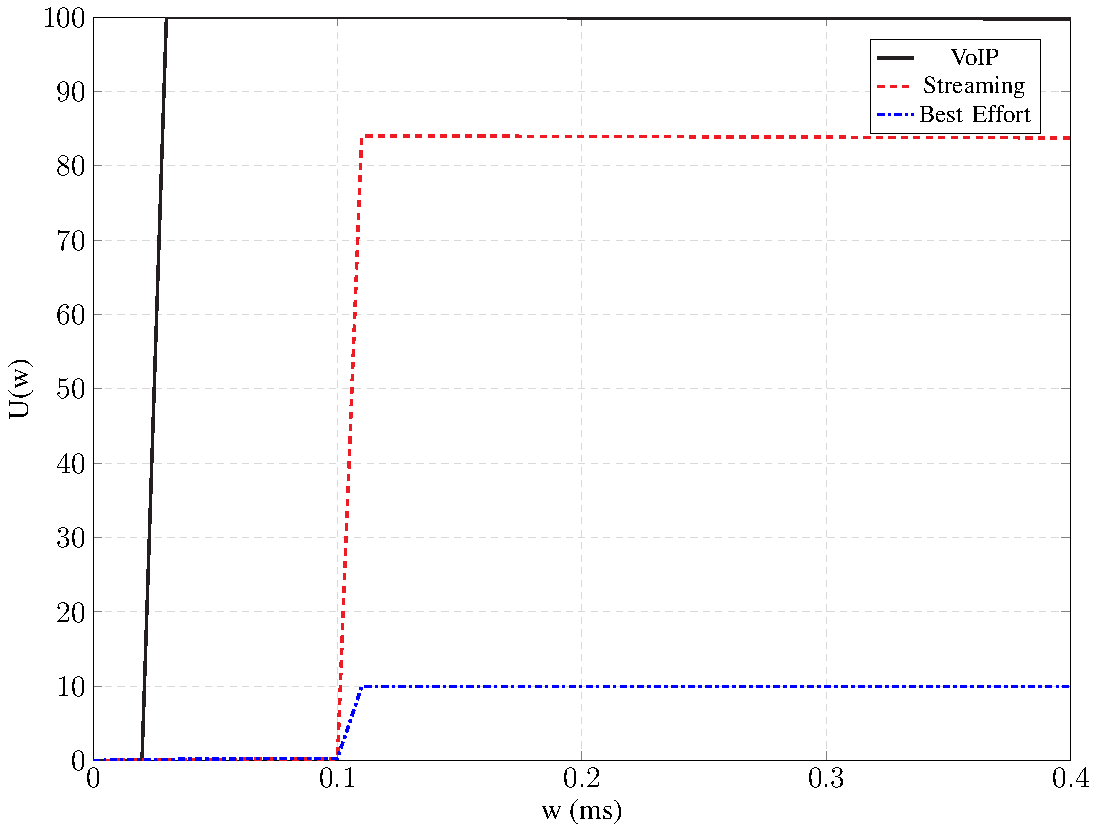
\includegraphics[width=0.8\textwidth]{figs/WeightsSongOriginal.pdf}
	
	{Fonte: Elaborada pelo autor.}
	\label{fig:WeightSong}
\end{figure} 

O autor então compara o desempenho do MDU com os algoritmos clássico PF, EXP e MLWDF, mostrando que o desempenho do MDU é melhor em termos de vazão de dados e atraso dos usuários.

\section{\textit{Utility} Lei}

O segundo algoritmo escolhido para um estudo mais aprofundado, implementação e análise de desempenho foi proposto em \citeonline{Proc:Lei2007}. Como já mencionado, iremos nos referir a este algoritmo como \textit{Utility} Lei. Este algoritmo foi proposto para a transmissão no enlace direto de sistemas celulares baseados em OFDMA compostos por serviços NRT e RT. Este algoritmo é baseado na CSI dos usuários e em uma função de utilidade com o atraso dos pacotes na fila de cada usuário como parâmetro.

Novamente, a teoria da utilidade é utilizada para a formulação do algoritmo de RRA. Além disso, as mesmas considerações adotas por \citeonline{song2004joint} em relação as características da função de utilidade são assumidas por \citeonline{Proc:Lei2007}. No entanto, a função de utilidade agora é baseada no atraso do pacote HOL do usuário $j$, ou seja, a função é da forma $U(d_{j}^{\text{hol}})$. Um problema de otimização é formulado com o objetivo de maximizar a utilidade total em cada TTI, ou seja, maximizar o somatório de $U(d_{j}^{\text{hol}})$.

Para obter a solução deste problema de otimização, os autores propuseram modelos para calcular os valores da vazão de dados dos usuários no TTI $n+1$ ($T_{j}\left[n+1\right]$) e atraso do pacote HOL no TTI $n+1$ $d_{j}^{\text{hol}}[n + 1]$. 

O modelo para calcular a vazão de dados do usuário $j$ utiliza um filtro exponencial para suavização, como indicado na equação 
%
\begin{equation}
\label{Eq:Thru}
T_{j}\left[n+1\right] = \left(1 - f_{\mathrm{thru}}\right) \cdot T_{j}\left[n\right] + f_{\mathrm{thru}} \cdot R_j\left[n\right],
\end{equation} 
%
em que $R_j\left[n\right]$ é a taxa instantânea de dados do usuário $j$ e $f_{\mathrm{thru}}$ é uma constante de filtragem similar a $f_{\mathrm{fila}}$ do algoritmo MDU. Este é o modelo de vazão de dados que é utilizado no ambiente de simulação deste trabalho.

O modelo para $d_{j}^{\text{hol}}[n + 1]$ é descrito pela equação 
%
\begin{equation}
\label{JSM:Eq:HOL_Delay}
d_{j}^\mathrm{hol}\left[n+1\right] = d_{j}^\mathrm{hol}\left[n\right] + \left( \frac{\theta_j\left[n\right] - R_j\left[n\right] \cdot t_{\mathrm{tti}}}{T_{j}\left[n\right]}\right),
\end{equation}
%
em que $\theta_j\left[n\right]$ é a quantidade de bits dos pacotes que chegaram na fila do usuário $j$ no TTI $n$ e $t_{\mathrm{tti}}$ é a duração do TTI.

A partir destes modelos e da função objetivo do problema de otimização formulado pelos autores, o usuário $j^{\star}$ é selecionado para transmitir no recurso $k$ durante o TTI $n$ de acordo com 
%
\begin{equation}
j^{\star} = \underset{j}{\text{arg max}}\Big\{ |U^{'}(d_{j}^{\text{hol}}[n])| \cdot \frac{r_{j, k}[n]}{T_{j}\left[n\right]} \Big \}, 
\end{equation}
%
em que $U^{'}(d_{j}^{\text{hol}}[n])$ denota a derivada primeira de $U(d_{j}^{\text{hol}}[n])$ em relação $d_{j}^{\text{hol}}[n]$.

As funções de utilidade escolhidas para definir a prioridade dos usuários durante o processo de alocação dos recursos foram
%
\begin{equation}
\label{Eq:MDU_RT}
U_{\text{RT}}(d_{j}^{\text{hol}}[n]) = 1 - (1 + e^{-\beta (d_{j}^{\text{hol}}[n] - \Phi_{\text{req}}^{\text{rt}})}),
\end{equation}
%
para o serviço RT (em que $\beta > 0$ determina a declividade da função e $\Phi_{\text{req}}^{\text{rt}} > 0$ determina o ponto de inflexão da função, que é definido como o tempo limite do pacote HOL) e para o serviço NRT, foi definida a função
%
\begin{equation}
U_{\text{NRT}}(d_{j}^{\text{hol}}[n]) = 1 - b \cdot e^{a \cdot  (d_{j}^{\text{hol}}[n] - c)},
\end{equation}
%
em que $a > 0$, $b > 0$, $c>0$. O valor de $a$ determina a declividade da função, $b$ determina a amplitude da função e $c$ normalmente é definido como o requerimento de QoS do serviço.

Essas duas funções são ilustradas na figura \ref{fig:PrimitiveWeightLEI} para os seguintes valores dos parâmetros, os quais foram propostos em \citeonline{Proc:Lei2007}: $\beta = 1.5$, $\Phi_{\text{req}}^{\text{rt}} = 5$, $a = 0.1$, $b = 0.5$ e $c = 10$. Note que as funções foram plotadas como função do atraso ($d_{j}^{\text{hol}}[n]$) em ms, diferentemente do que foi originalmente mostrado em \citeonline{Proc:Lei2007}. Os valores do eixo das abscissas não refletem exatamente os valores do $d_{j}^{\text{hol}}[n]$ que são obtidos durante a simulação. O objetivo aqui é apenas ilustrar o formato das funções utilizadas. 

\begin{figure}[ht]
	\centering	
	
	\caption[Funções de utilidade para os serviços RT e NRT]{Funções de utilidade para os serviços RT e NRT.}
	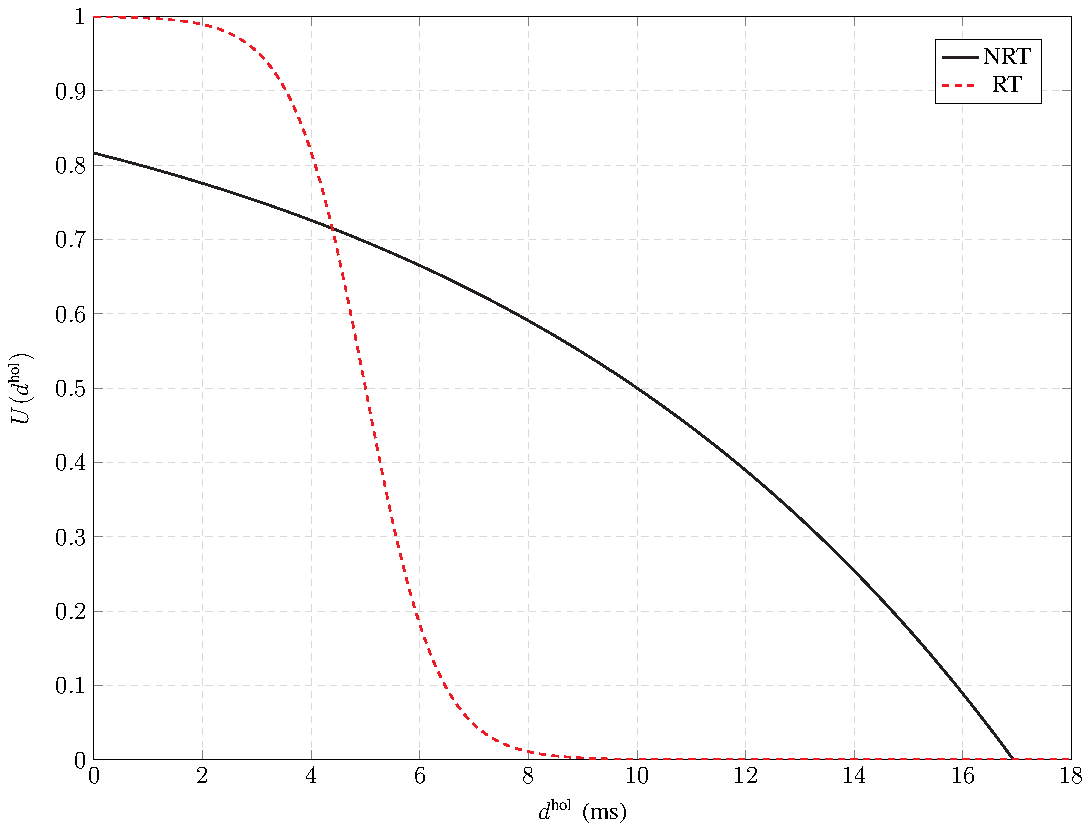
\includegraphics[width=0.8\textwidth]{figs/PrimitiveWeightLEIOriginal.pdf}
	
	{Fonte: Elaborado pelo autor, baseado em \cite{Proc:Lei2007}.}
	\label{fig:PrimitiveWeightLEI}
\end{figure} 

Para calcular a prioridade dos usuários durante a alocação dos recursos, é necessário calcular a primeira derivada dessas duas funções. Após este processo, obtêm-se as seguintes funções:
%
\begin{equation}
\label{Eq:LeiMarginalRT}
U^{'}_{\text{RT}}(d_{j}^{\text{hol}}[n]) =	\dfrac{ \beta  e^{-\beta (d_{j}^{\text{hol}}[n] - \Phi_{\text{req}}^{\text{rt}})}}{\left(1 + e^{\beta (d_{j}^{\text{hol}}[n] - \Phi_{\text{req}}^{\text{rt}})}\right)^{2}}
\end{equation}
%
\begin{equation}
U^{'}_{\text{NRT}}(d_{j}^{\text{hol}}[n]) = 	\text{a}\cdot \text{b}\cdot e^{\text{a}(d_{j}^{\text{hol}}[n]- c)}
\end{equation}

O formato destas funções está ilustrado na figura \ref{fig:WeightLEI}. A mesma observação em relação ao eixo das abscissas para a figura \ref{fig:PrimitiveWeightLEI} vale para a figura \ref{fig:WeightLEI}. Pode-se perceber que para valores de $t$ próximos do valor do requerimento de QoS do serviço RT, a prioridade deste serviço é maior que a prioridade do serviço NRT. Para valores mais distantes deste valor de requerimento, o serviço NRT tem prioridade maior.

\begin{figure}[ht]
	\centering	
	
	\caption[Derivada primeira das funções de utilidade para os serviços RT e NRT]{Derivada primeira das funções de utilidade para os serviços RT e NRT.}
	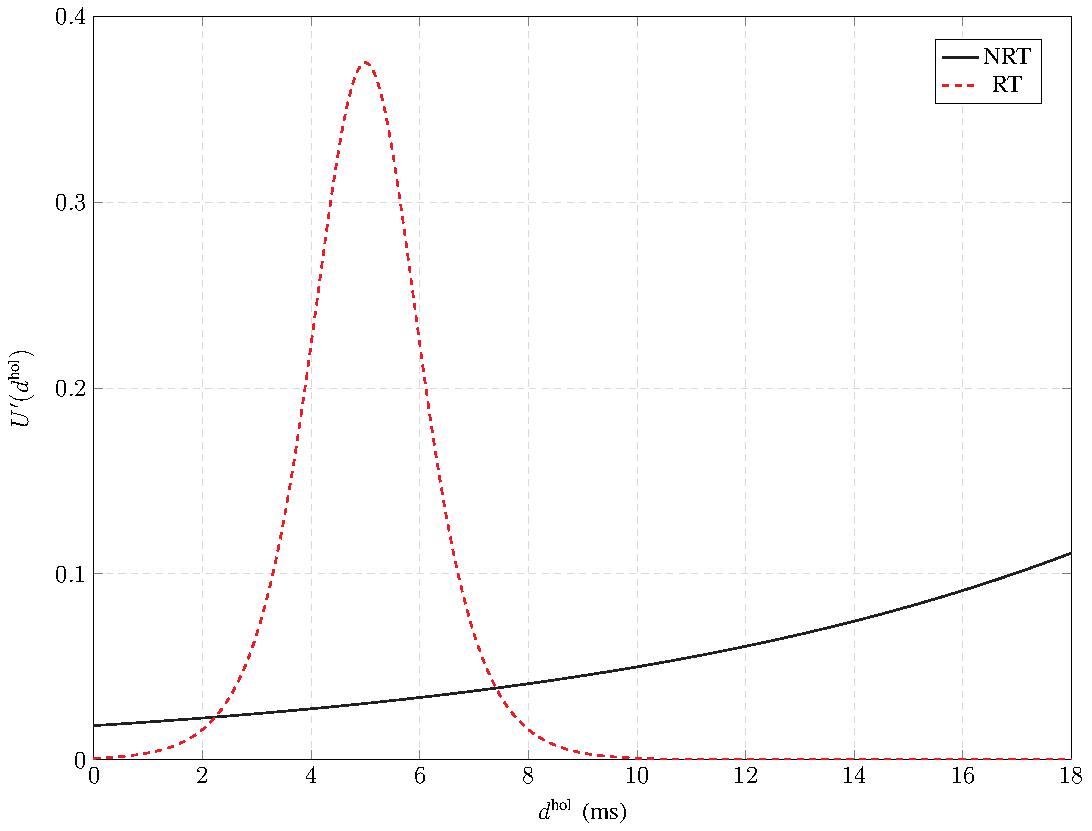
\includegraphics[width=0.8\textwidth]{figs/MarginalWeightLEIOriginal.pdf}
	
	{Fonte: Elaborado pelo autor, baseado em \cite{Proc:Lei2007}.}
	\label{fig:WeightLEI}
\end{figure} 

O desempenho deste algoritmo foi comparado com o desempenho dos algoritmos EXP, PF e MLWDF. Os autores mostraram que o \textit{Utility} Lei proporciona melhor desempenho em relação a vazão de dados e PLR. No entanto, o desempenho em relação a justiça na alocação dos recursos do \textit{Utility} Lei não foi melhor que o desempenho dos outros algoritmos.   

\section{\textit{Queue}-HOL-MLWDF (QHMLWDF)}

O terceiro algoritmo de RRA estudado com mais detalhes neste trabalho foi proposto em \citeonline{Nasralla2013}, o qual tenta garantir uma justa alocação dos recursos entre os serviços presentes no sistema.

Diferentemente do MDU e \textit{Utility} Lei, o QHMLWDF não possui uma formulação matemática com um problema de otimização. Este algoritmo é apresentado como uma versão modificada/melhorada baseada em outros dois algoritmos, a saber MLWDF$^{2}$\footnotetext[2]{O algoritmo MLWDF foi inicialmente proposto por \citeonline{Art:Andrews2001}. No entanto, em \citeonline{Nasralla2013}, os autores consideram uma versão modificada apresentada em \citeonline{ameigeiras2004performance}} \cite{ameigeiras2004performance} e \ac{VTMLWDF} \cite{iturralde2011performance}.

O algoritmo MLWDF foi concebido para suportar serviços de multimídia \cite{Nasralla2013}. Em \citeonline{ameigeiras2004performance}, os autores mostram que este algoritmo apresenta desempenho melhor que outros algoritmos de RRA para cenários com serviços de vídeo. A versão do MLWDF estudada em \citeonline{ameigeiras2004performance} aloca recursos para o serviço RT baseado-se no atraso do pacote HOL, a saber
%
\begin{equation}
j^{\star} = \underset{j}{\text{arg max}}\Big\{ \dfrac{\alpha[n] \cdot d_{j}^{\text{hol}}[n] } {T_{j}[n]} \cdot r_{j, k}[n] \Big \},
\end{equation}
%
em que $\alpha[n]$ representa a máxima probabilidade permitida que os pacotes excedam o tempo limite pré-estabelecido. Os recursos são alocados para o serviço NRT a partir da política de alocação de recursos do algoritmo PF, que é
%
\begin{equation}
\label{eq:PF}
j^{\star} = \underset{j}{\text{arg max}}\Big\{\frac{r_{j, k}[n]}{T_{j}\left[n\right]} \Big \}.
\end{equation}

O algoritmo VTMLWDF \cite{iturralde2011performance} tem o objetivo de priorizar o serviço RT e, ao mesmo tempo, tentar garantir os requerimentos de serviços NRT. O escalonamento dos recursos é baseado principalmente no tamanho da fila de pacotes do usuário, o que, segundo os autores, ajuda a alocar a maioria dos recursos para usuários de vídeo, penalizando os usuários NRT. Para o serviço RT, a política utilizada para a alocação é 
%
\begin{equation}
j^{\star} = \underset{j}{\text{arg max}}\Big\{ \dfrac{\alpha[n] \cdot \text{Q}_{j}[n]} {T_{j}[n]} \cdot r_{j, k}[n] \Big\},
\end{equation}
%
em que $\text{Q}_{j}[n]$ representa o tamanho da fila de pacote (em bits) do usuário $j$. Para o serviço NRT, a política de alocação dos recursos está descrita na equação \ref{eq:PF}. 

O algoritmo QHMLWDF combina, segundo \citeonline{Nasralla2013}, o uso das principais métricas utilizadas no MLWDF e VTMLWDF: 1) o atraso do pacote HOL, que ajuda na alocação dos recursos para usuários com atraso perto do tempo limite; 2) o tamanho da fila de pacote, que quantifica a prioridade dos serviços de acordo o tamanho em bits da fila. Além disso, a proposta do QHMLWDF utiliza apenas uma fórmula para alocar os recursos para as diferentes classes de serviço. Neste algoritmo, o usuário $j^{\star}$ é selecionado para transmitir no recurso $k$ durante o TTI $n$ de acordo com 
%
\begin{equation}
\label{Eq:QHMLWDF_RT_NRT}
j^{\star} = \underset{j}{\text{arg max}}\Big\{ \dfrac{\alpha[n] \cdot d_{j}^{\text{hol}}[n] \cdot \text{Q}_{j}[n]} {T_{j}[n]} \cdot r_{j, k}[n] \Big\},
\end{equation}
%
que vale para os serviços RT e NRT.

Como o algoritmo QHMLWDF foi uma evolução/modificação dos algoritmos MLWDF e VTMLWDF, o autor faz a comparação de desempenho com estes algoritmos. O algoritmo QHMLWDF mostrou algumas melhoras em termos de algumas métricas de QoS, tais como PLR, vazão de dados média, justiça e eficiência espectral, considerando um cenário composto por três serviços, a saber vídeo, VoIP e \textit{Best Effort}.

\section{\textit{Exponential}/\textit{Proportional Fair} (EXP/PF)}

O algoritmo de RRA conhecido como EXP/PF foi originalmente concebido por \cite{rhee2003scheduling} para suportar aplicações de multimídia em sistemas com multiplexação no tempo. Os autores visavam garantir que os serviços RT conseguissem transmitir dentro de um determinando limite de tempo e que a vazão de dados do sistema fosse maximizado. Em \citeonline{basukala2009performance}, os autores adaptaram este algoritmo para sistema baseados em OFDMA, como por exemplo os sistemas celulares 4G LTE, onde foi mostrado que este algoritmo tem um desempenho melhor que o algoritmo MLWDF.  

A alocação dos recursos para o serviço RT é feita utilizando o algoritmo EXP, que foi inicialmente concebido para sistemas \ac{CDMA} com uma única portadora e com o espectro do enlace direto compartilhado  \cite{shakkottai2002scheduling}. A fórmula para \citeonline{shakkottai2002scheduling} decidir qual usuário será selecionado para transmitir no RB $k$ no TTI $n$ para um cenário com múltiplos canais é
%
\begin{equation}
\label{Eq:EXPPF_RT}
j^{\star} = \underset{j}{\text{arg max}}\left\{ \text{exp}\left(\dfrac{d_{j}^{\text{hol}}[n]}{1 + \sqrt{\overline{d_{j}^{\text{hol}}}[n]}}\right) \cdot \dfrac{r_{j, k}[n]}{T_{j}[n]} \right\}
\end{equation}
%
em que $\overline{d_{j}^{\text{hol}}}[n]$ é a média do atraso dos pacotes HOL de todos os usuários RT ativos no TTI $n$. Perceba que a partir desta fórmula, o algoritmo tenta garantir que os usuários de serviços RT consigam transmitir rapidamente após ficarem ativos. A medida que o atraso do pacote HOL de um usuário $j$ se distancia da média $\overline{d_{j}^{\text{hol}}}[n]$, sua prioridade aumenta.

Para o serviço NRT, o EXP/PF aloca os recursos segundo a política do algoritmo PF, que é dada pela equação
%
\begin{equation}
\label{Eq:EXPPF_NRT}
j^{\star} = \underset{j}{\text{arg max}}\Big\{\frac{r_{j, k}[n]}{T_{j}\left[n\right]} \Big \},
\end{equation}

O algoritmo PF aloca os recursos para os usuários com boas condições de canal e consegue garantir uma boa vazão de dados total do sistema e consideravelmente bons níveis de justiça na alocação dos recursos.


